%% lineno required for submission for peer review
\documentclass[fleqn,10pt,lineno]{wlpeerj} % for journal submissions
% \documentclass[fleqn,10pt]{wlpeerj} % for preprint submissions

\newcommand{\comment}[1]{}

\usepackage{array}
\usepackage{hyperref}
\usepackage{siunitx}
\newcommand{\hlcell}[1]{\textbf{#1}}

\newcolumntype{L}[1]{>{\raggedright\let\newline\\\arraybackslash\hspace{0pt}}m{#1}}
\newcolumntype{C}[1]{>{\centering\let\newline\\\arraybackslash\hspace{0pt}}m{#1}}
\newcolumntype{R}[1]{>{\raggedleft\let\newline\\\arraybackslash\hspace{0pt}}m{#1}}

\title{Supplement to \textit{Atropos: specific, sensitive, and speedy trimming of sequencing reads}}

\author[1]{John P Didion}
\author[2]{Marcel Martin}
\author[1]{Francis S Collins}
\affil[1]{National Human Genome Research Institute, National Institutes of Health, Bethesda, MD}
\affil[2]{Science for Life Laboratory, Department of Biochemistry and Biophysics,
Stockholm University, Sweden}
\corrauthor[1]{John P Didion, PhD}{john.didion@nih.gov}

\begin{abstract}
\end{abstract}

\begin{document}

\flushbottom
\maketitle
\thispagestyle{empty}
\section{Figures}

\begin{figure}[!ht]
\centering
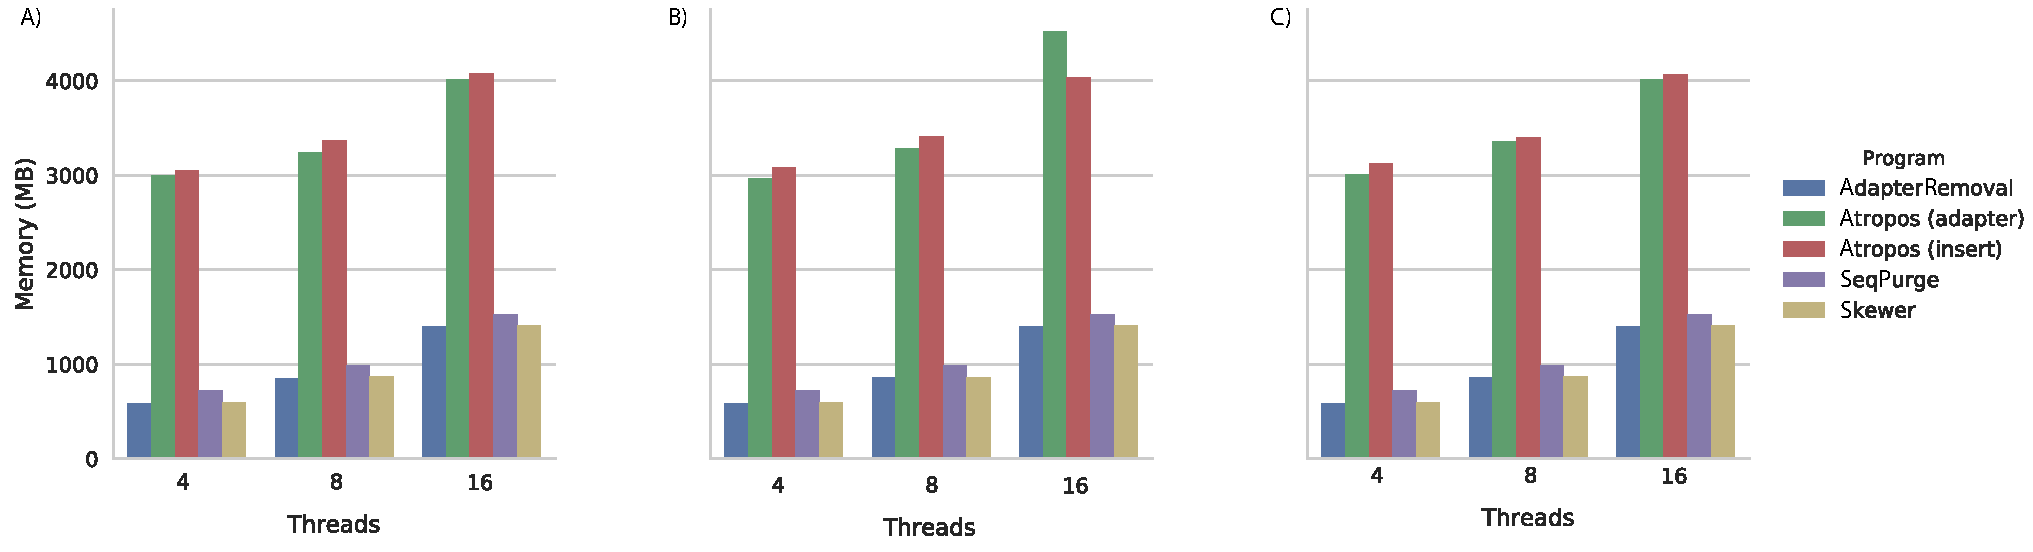
\includegraphics[width=\linewidth]{FigureS1.pdf}
\caption{\textbf{Memory usage of trimming tools on simulated datasets.} Maximum memory usage, in MB, of jobs executed on our cluster for trimming tools run on simulated datasets with error rates of A) 0.2\%, B) 0.6\%, and C) 1.2\%. Note that this memory usage includes the overhead of the Singularity container and is thus an overestimate.}
\label{fig:memory}
\end{figure}

\begin{figure}[!ht]
\centering
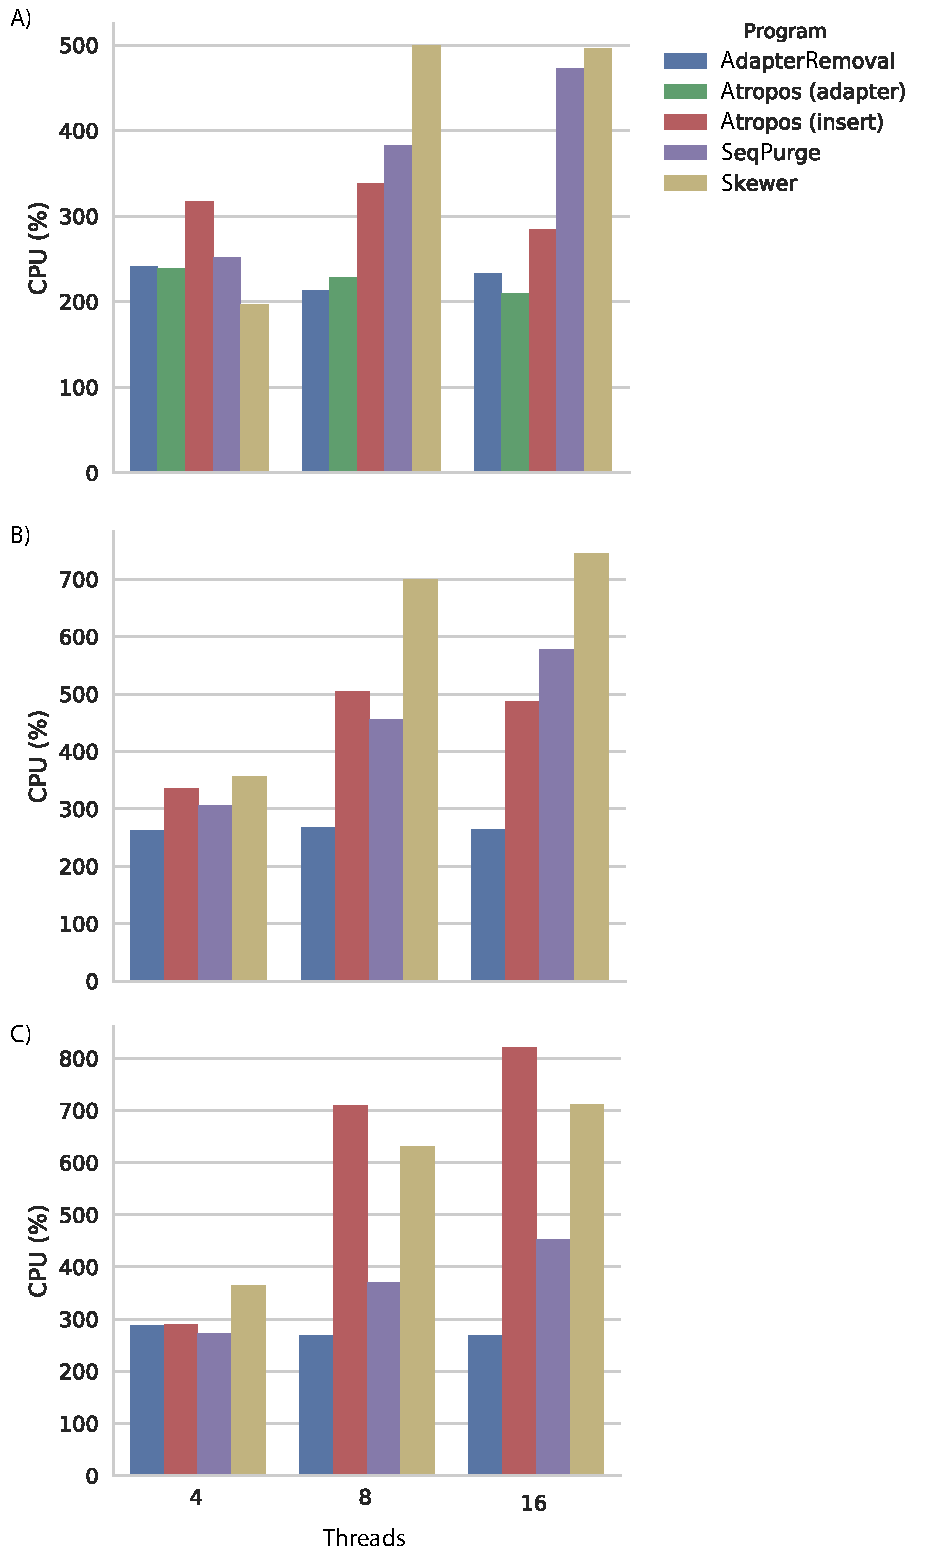
\includegraphics[width=4in]{FigureS2.pdf}
\caption{\textbf{CPU Utilization of trimming tools.} Average total CPU usage of each trimming tool run on A) simulated data, B) WGBS data, and C) mRNA-Seq data.}
\label{fig:cpu}
\end{figure}

\begin{figure}[!ht]
\centering
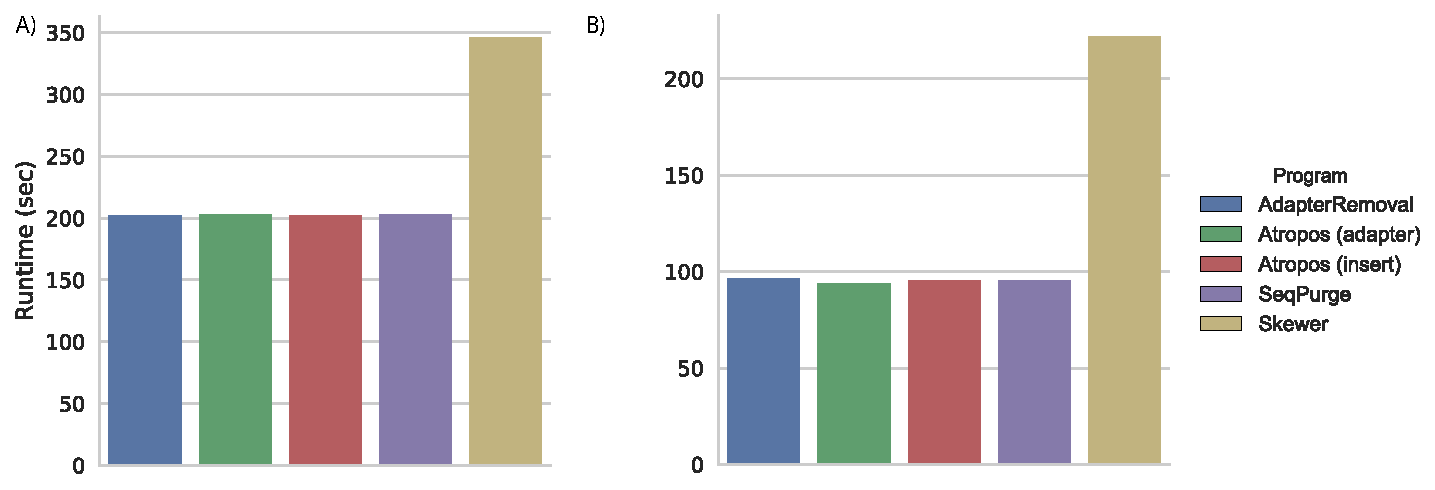
\includegraphics[width=\linewidth]{FigureS3.pdf}
\caption{\textbf{Mapping execution times.} Execution time of A) bwa-meth on WGBS reads, and B) STAR on mRNA-Seq reads, for reads trimmed by each tool as well as the untrimmed reads.}
\label{fig:mapping}
\end{figure}

\clearpage

\section{tables}

\input{containers.tex}

\input{simulated_performance_local.tex}

\input{simulated_performance_cluster.tex}

\input{memory.tex}

\input{real_performance_wgbs.tex}

\input{real_performance_rnaseq.tex}
\clearpage
\bibliography{Zotero,marcel}

\end{document}